%!TEX root = ../report_template.tex
\section{Methods}
The basis of the exploratory data analysis are the used datasets and the applied mathematical concepts for forming a quantitative argumentation. Thus, this section first introduces the used data sets and explains afterward the mathematical background. Finally, this section analyzes first trends and findings on the effects of increasing grades.

\subsection{Datasets}
This paper investigates both the causes and effects of the phenomena discussed in \autoref{sec:Introduction}. Thus, the analyzed datasets are grouped into \emph{cause} and \emph{effect} datasets. All used datasets are collected on all public schools, since they are obliged to forward the federal statistical institutions \cite{statistische_bundesamt_statistisches_2024,kultusminister_konferenz_abiturnoten_nodate}.

In the following, \emph{causes} are defined as the social, demographic, or political factors that  influence the German school system, such as the number of students, teachers, or budget provided by the German government. In contrast, \emph{effect} refers to the observable impact of these causes on any measure modeling the students' performance, e.g., average grades or the rate of repeaters and school-leavers.

% Causes
The first dataset is the \textit{Fachreport Schuljahr 2020/21} presenting the number of teachers from 1992 until 2020 \cite{statistische_bundesamt_allgemeinbildende_2022}. The dataset is grouped into contract type, federal state, and school type. In addition, the count of schoolchildren is analyzed with two datasets \cite{statistische_bundesamt_statistisches_2024}. The first dataset (\href{https://www-genesis.destatis.de/genesis//online?operation=table&code=21111-0002&bypass=true&levelindex=0&levelid=1706352545984#abreadcrumb}{$21111-0002$}) contains the number of children per grade and school type  for the years 1998 to 2022. In contrast, the second (\href{https://www-genesis.destatis.de/genesis//online?operation=table&code=21111-0010&bypass=true&levelindex=0&levelid=1706352536762#abreadcrumb}{$21111-0010$}) provides the absolute number of children, leavers, and beginners in each federal state from 1997 to 2022. Therefore, the analysis can only be conducted separately for school types and federal states, due to the missing representation.

Additionally, this paper considers the budget per child (\href{https://www-genesis.destatis.de/genesis//online?operation=table&code=21711-0011&bypass=true&levelindex=0&levelid=1706352648560#abreadcrumb}{$21711-0011$}) as a possible cause, which is provided  by the \citeauthor{statistische_bundesamt_statistisches_2024}. The dataset contains the budget per child for the years 2010 to 2022 and is grouped by federal states. To adjust for inflation, the budget is multiplied with the \textit{Verbraucherpreisindex} (\href{https://www-genesis.destatis.de/genesis//online?operation=table&code=61111-0010&bypass=true&levelindex=0&levelid=1706352769529#abreadcrumb}{$61111-0010$}) relative to 2022, as provided by the \citeauthor{statistische_bundesamt_statistisches_2024}. 


% Effects
It is also important to analyze the  effects on student performance, since they are the first indicator of whether grade inflation exists. One of the few publicly available datasets containing grades is the average Abitur grades per federal state. The grades are published every year in a separate report by the \citeauthor{kultusminister_konferenz_abiturnoten_nodate}. Each file contains the count of children per written grade and federal state. The grades are given in increments of $0.1$, with $4.0$  being the worst and $1.0$ being the best grade. The number of children who failed with a grade worse than $4.0$ is aggregated in an additional column. 

Although this is a great model for the performance of children attending grammar schools, a general performance measure for all school types is required to translate the results to all school types. Accordingly, this paper uses the number of repeaters (\href{https://www-genesis.destatis.de/genesis//online?operation=table&code=21111-0014&bypass=true&levelindex=0&levelid=1706352887288#abreadcrumb}{$21111-0014$}) from the \citeauthor{statistische_bundesamt_statistisches_2024}. There, the absolute count of repeaters by federal state, school type, and year is provided for the years 1998 to 2022.

\subsection{Mathematical Concepts}
The subsequent paragraph provides an overview of two concepts: linear regression and the Pearson correlation coefficient.

Firstly, linear regression is a statistical technique for modeling the relationship between a dependent variable and one or more independent variables \cite{james_introduction_2021}. It seeks to fit a linear equation to the data that minimizes the discrepancy between observed and predicted values. This is done through least squares minimization, resulting in an equation of the form \cite{james_introduction_2021}:
\begin{equation}
    Y = \beta_0 + \beta_1 X_1 + \beta_2 X_2 +  ...+ \beta_p X_p + \epsilon 
\end{equation}

Finally, the Pearson correlation coefficient $r$, is a statistical measure used to assess the linear relationship between two sets of data, $X$ and $Y$ \cite{rodgers_thirteen_1988}. It is computed as the ratio of the sample covariance of $X$ and $Y$ to the product of their sample standard deviations \cite{rodgers_thirteen_1988}:
\begin{equation}
    r = \frac{\sum_{i=1}^n (X_i - \overline{X}) (Y_i - \overline{Y})}{\sqrt{\sum_{i=1}^n(X_i-\overline{X})^2 \cdot \sum_{i=1}^n(Y_i-\overline{Y})^2}}
\end{equation}

\subsection{Exploratory Data Analysis}
Having introduced all used datasets, this paragraph aims to investigate potential patterns through an exploratory data analysis of the potential \emph{causes} and \emph{effects}. 

% Describe causes
% Todo: Sources
Firstly, regard the demographic effects on the number of children attending school and teachers employed by school type and federal state. The exploratory data analysis of the teachers and children datasets\footnote{\label{footnote:teachers-children}Teachers and children plots and exploration can be found \href{https://github.com/KarylReyne/DataLiteracyWS23/blob/main/exp/TF-005-TeachersToChildren.ipynb}{here}.} has shown that the number of schoolchildren decreases steadily from 1998 to 2014. Instead, it increased from 2019 to 2022 because more children started their education and fewer left school. Furthermore, more children graduate from grammar schools with university entrance qualifications. This demographic effect is combined with an increasing number of teachers across all German school types and federal states. Although, the percentage of part-time teachers is increasing, the number of full-time teachers is decreasing until 2020.

\begin{figure*}[ht!]
    \centering
    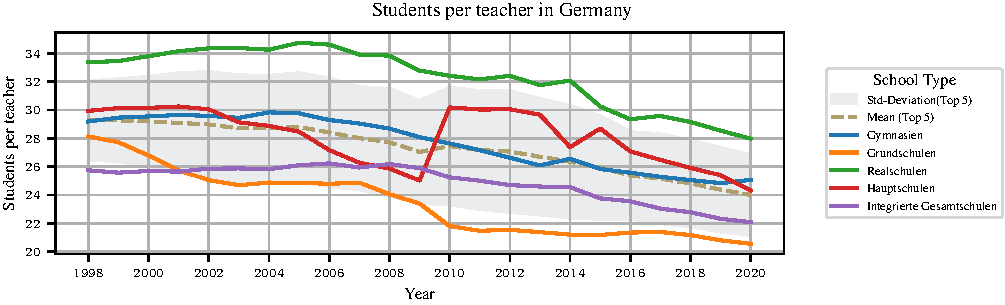
\includegraphics{fig/fig_students_per_teacher_per_school_type.pdf}
    \caption{Student-to-teacher ratio of the five most common school types in Germany. The ratio of full- and part-time teachers is displayed for each school type and aggregated to their average (\textcolor{TUgold}{\rule[-0.2ex]{0.5em}{2pt} \rule[-0.2ex]{0.5em}{2pt}}).}
    \label{fig:spt-type}
\end{figure*}

Given the hypothesis that having more teachers per student increases the quality of teaching, the datasets are merged \cite{kasau_onesmus_mulei_pupil-teacher_2016,koc_impact_2015}. As already explained, this merge can only been done separately for school types and federal states. Furthermore, the student-to-teacher ratio is calculated over all full- and part-time teachers, since they represent the majority ({\raise.17ex\hbox{$\scriptstyle\mathtt{\sim}$}} $90\%$) of the distribution\footref{footnote:teachers-children}. In contrast, the teachers who are employed on an hourly basis are excluded due to their small impact on the teaching quality and sparse representation in the data. The results in \autoref{fig:spt-type} show that from 1998 to 2020, the ratio decreased for the five most common school types. As a result, the average decreases from 29 to 24 children per teacher. Together with the hypothesis, it follows that the quality of teaching should increase, and thus the performance measures should increase.

Besides the demographic measures, the analysis of the adjusted budget\footnote{\label{footnote:budget}Budget plots and exploration can be found \href{https://github.com/KarylReyne/DataLiteracyWS23/blob/main/exp/TF-007-SchoolBudgets.ipynb}{here}.} to inflation per child has shown that it steadily increases for all federal states. Although, this may be caused by the increasing number of teachers and the goals of digitalization of schools in the last years \cite{cone_pandemic_2022}.

% Effects
Now that some basic effects that may influence the students' performance have been identified, it is possible to study the performance measures. As the analysis of the students datasets\footref{footnote:teachers-children} has shown, more children are attending grammar schools in Germany. Thus, the average Abitur grade of the children is a great measure of the performance of many children. The analysis results of the Abitur grades\footnote{\label{footnote:abi}Abitur plots and exploration can be found \href{https://github.com/KarylReyne/DataLiteracyWS23/blob/main/exp/TF-001-ExploreABIGrades.ipynb}{here}.} are shown in \autoref{fig:rising-grades}. Importantly, the regression is calculated on the data before 2021 because of the COVID-19 pandemic beginning in 2020. In 2022, the grades significantly increased compared to the years before the pandemic. This could indicate that the pandemic has had novel consequences for the educational system. Due to the lack of data following the pandemic, this paper will solely focus on the linear trend until 2020. Furthermore, an additional analysis\footref{footnote:abi} of the relative number of failed students has shown that the failure rate has no repetitive or linear pattern. Therefore, the provided results in \autoref{fig:rising-grades} are only valid for children graduating with a grade of at least 4.0.

\begin{figure}[ht]
    \centering
    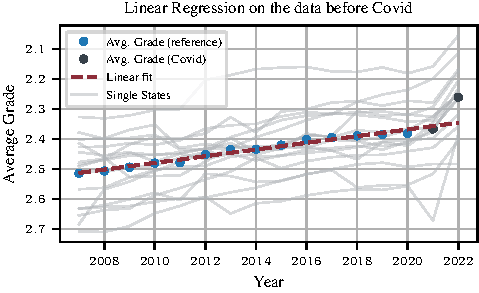
\includegraphics{fig/fig_rising_grades.pdf}
    \caption{Average Abitur grades before (\textcolor{TUlightblue}{\tikz\draw[fill={TUlightblue}] (0,0) circle (0.25em);}) and after the COVID-19 pandemic (\textcolor{TUdark}{\tikz\draw[fill={TUdark}] (0,0) circle (0.25em);}) with a linear regression line (\textcolor{TUred}{\rule[-0.2ex]{0.5em}{2pt} \rule[-0.2ex]{0.5em}{2pt}}) of the years 2007 to 2020. In the background the figure contains average grades for each federal state (\textcolor{TUgray}{\rule[-0.2ex]{0.5em}{1pt}}).}
    \label{fig:rising-grades}
\end{figure}

Moreover, all children attending other schools have no direct impact on the results of the Abitur grades. Therefore, the number of repeaters per federal state, school type, grade, and school year is analyzed. To enhance the relevance of the results, the relative ratio of repeaters\footnote{\label{footnote:repeaters}Repeater plots and exploration can be found \href{https://github.com/KarylReyne/DataLiteracyWS23/blob/main/exp/JS-001-Repeaters.ipynb}{here}.} is calculated by dividing the absolute counts by the absolute number of schoolchildren. This results in an aggregation for the federal states per year and in one for the school types per year. As a result, the number of repeaters has decreased for all educational institutions and federal states from 1998 to 2020. Hence, the trend equals the expected result, after analyzing the Abitur grades.

To summarize, the exploratory findings indicate an increasing number of students and teachers, resulting in a decreasing ratio of students to teachers and a rise in the budget per child. The possible outcomes include a linear increase in Abitur grades in grammar schools and a shrinking proportion of repeaters in general.
